% -*- mode: noweb; noweb-default-code-mode: R-mode; -*-
\documentclass[a4paper]{article}
\usepackage[margin=0.5in]{geometry}
\usepackage{/Library/Frameworks/R.framework/Resources/share/texmf/Sweave}


\title{R Code for Modelling Gasification and Related Processes}
\author{Bear Kaufmann\\
\normalsize{All Power Labs}\\
\normalsize{1010 Murray St., Berkeley, CA}\\
\normalsize{bear@allpowerlabs.org}
}

\begin{document}
\maketitle
\vfill
\begin{center}

\includegraphics[width=1in]{images/cc_by_sa.png}\\
This document and associated code is released as Creative Commons Attribution - Share Alike.
For more information on this license, please visit http://creativecommons.org/about/licenses/
\end{center}
\newpage
\section{Description}
The code here is used to help in modelling gasification reactions and related processes. 

\section{Graphs}
\subsection{Gasification Gas Composition vs. Lambda}
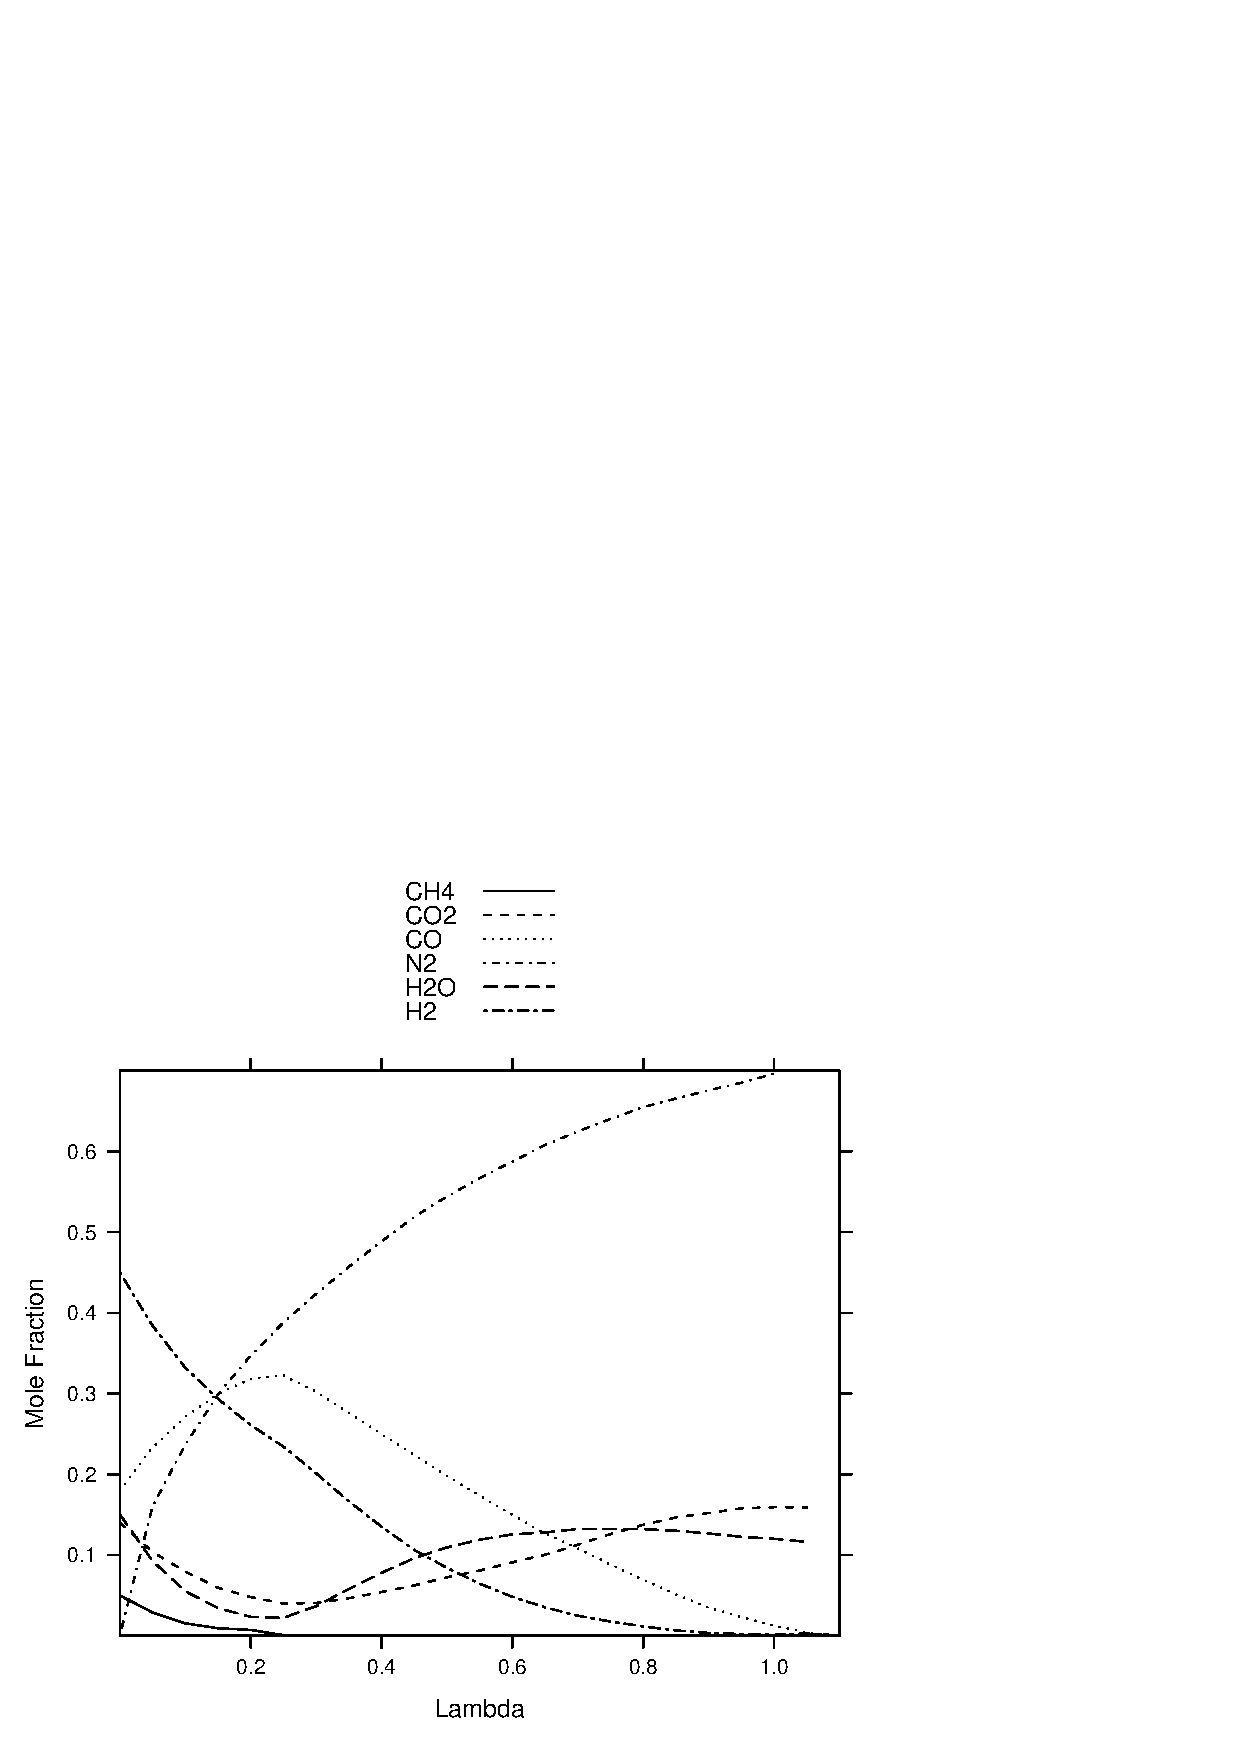
\includegraphics{images/img-001}
\\
\section{Van Krevelen Diagram}
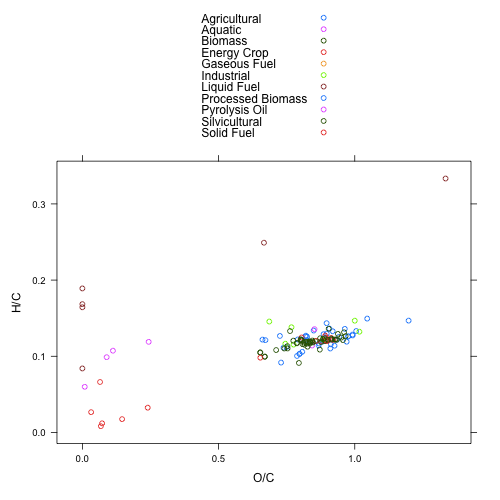
\includegraphics{images/img-002}
\\
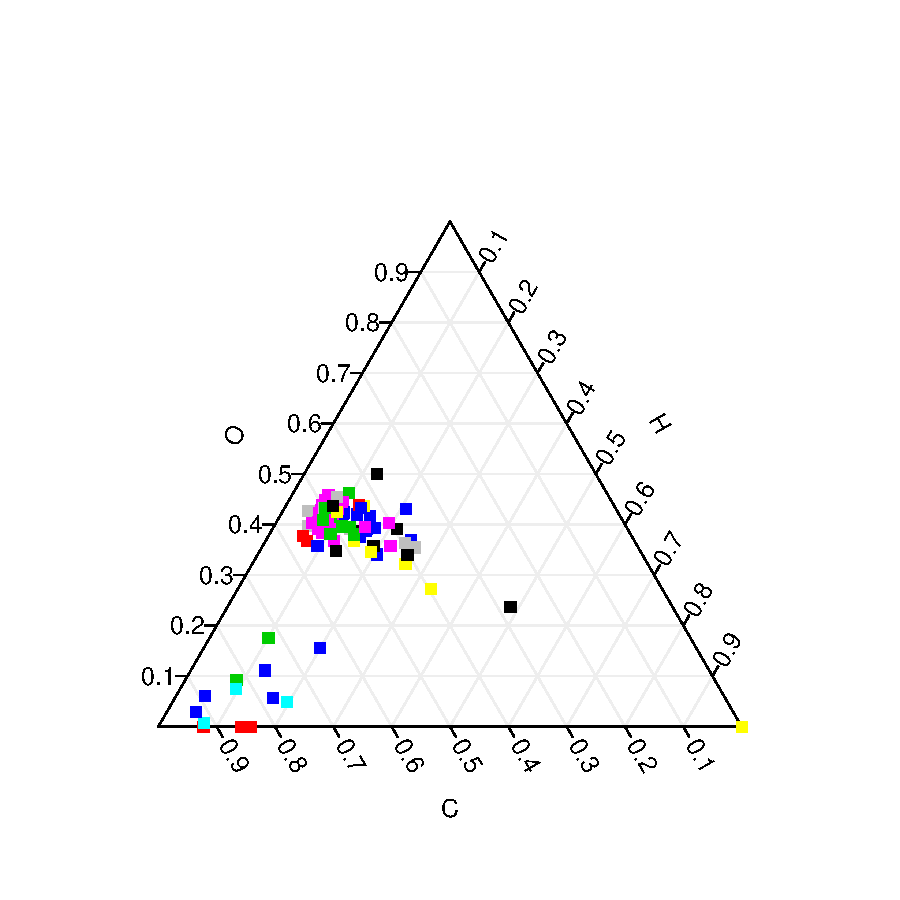
\includegraphics{images/img-003}
\\
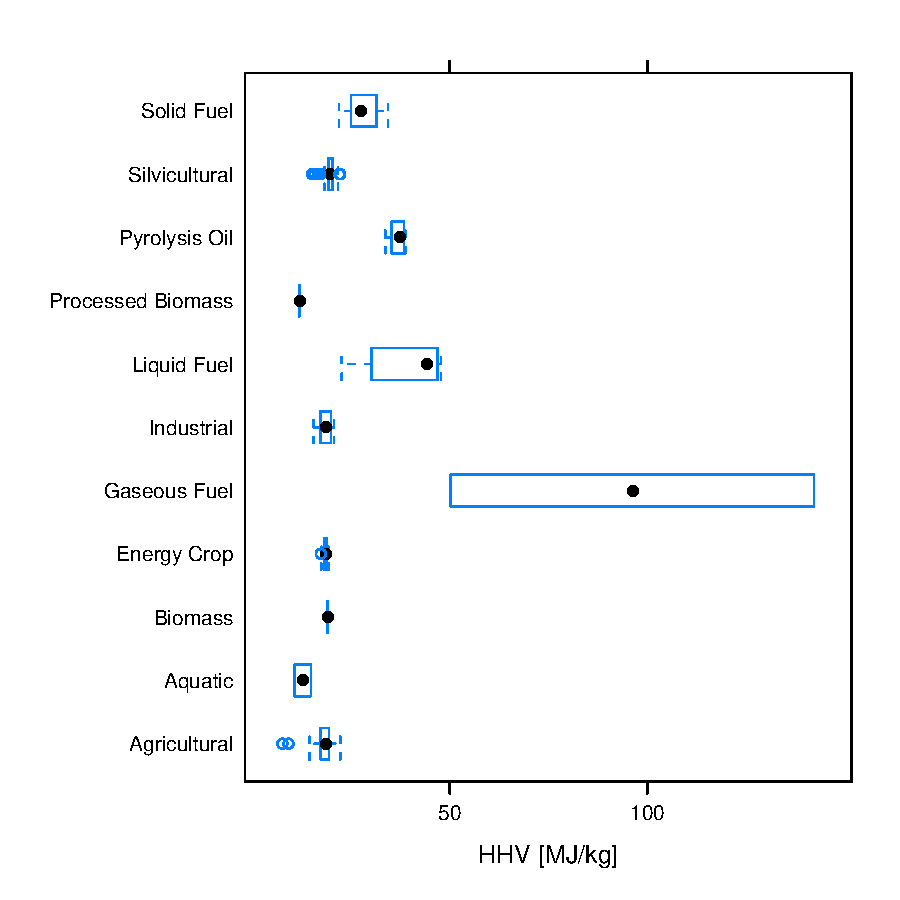
\includegraphics{images/img-004}
\\
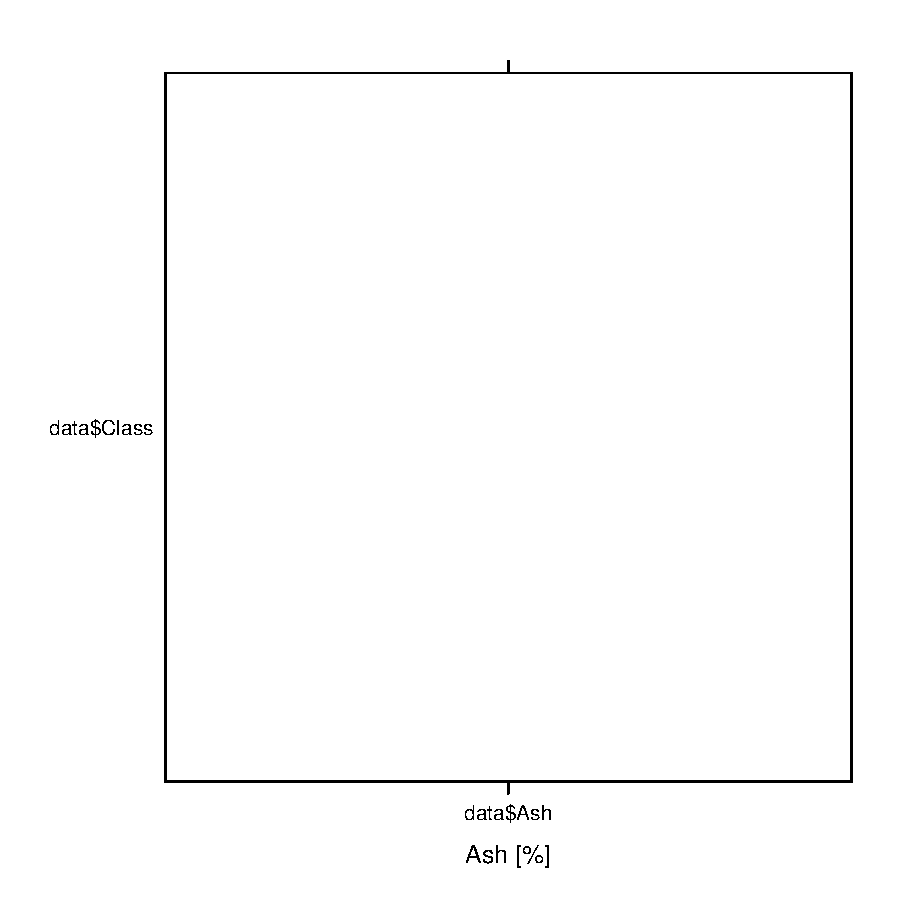
\includegraphics{images/img-005}
\\
% latex table generated in R 2.11.1 by xtable 1.5-6 package
% Wed Jan  5 01:46:21 2011
\begin{table}[ht]
\begin{center}
\begin{tabular}{rllrrrrrrrrrrrl}
  \hline
 & Class & Entity & Fixed.Carbon & Volatiles & Ash & C & H & O & N & S & Cl & HHV\_meas & HHV\_calc & Source \\ 
  \hline
87 & Aquatic Biomass & Water Hyacinth (Florida) &  & 80.40 & 19.60 & 40.30 & 4.60 & 33.99 & 1.51 & 0.00 &  & 14.86 & 15.54 & http://www.woodgas.com/proximat.htm \\ 
  88 & Aquatic Biomass & Brown Kelp,Giant, Soquel Point &  & 57.90 & 42.10 & 27.80 & 3.77 & 23.69 & 4.63 & 1.05 &  & 10.75 & 10.85 & http://www.woodgas.com/proximat.htm \\ 
   \hline
\end{tabular}
\caption{Data for Aquatic Biomass}
\end{center}
\end{table}
\section{Combustion}
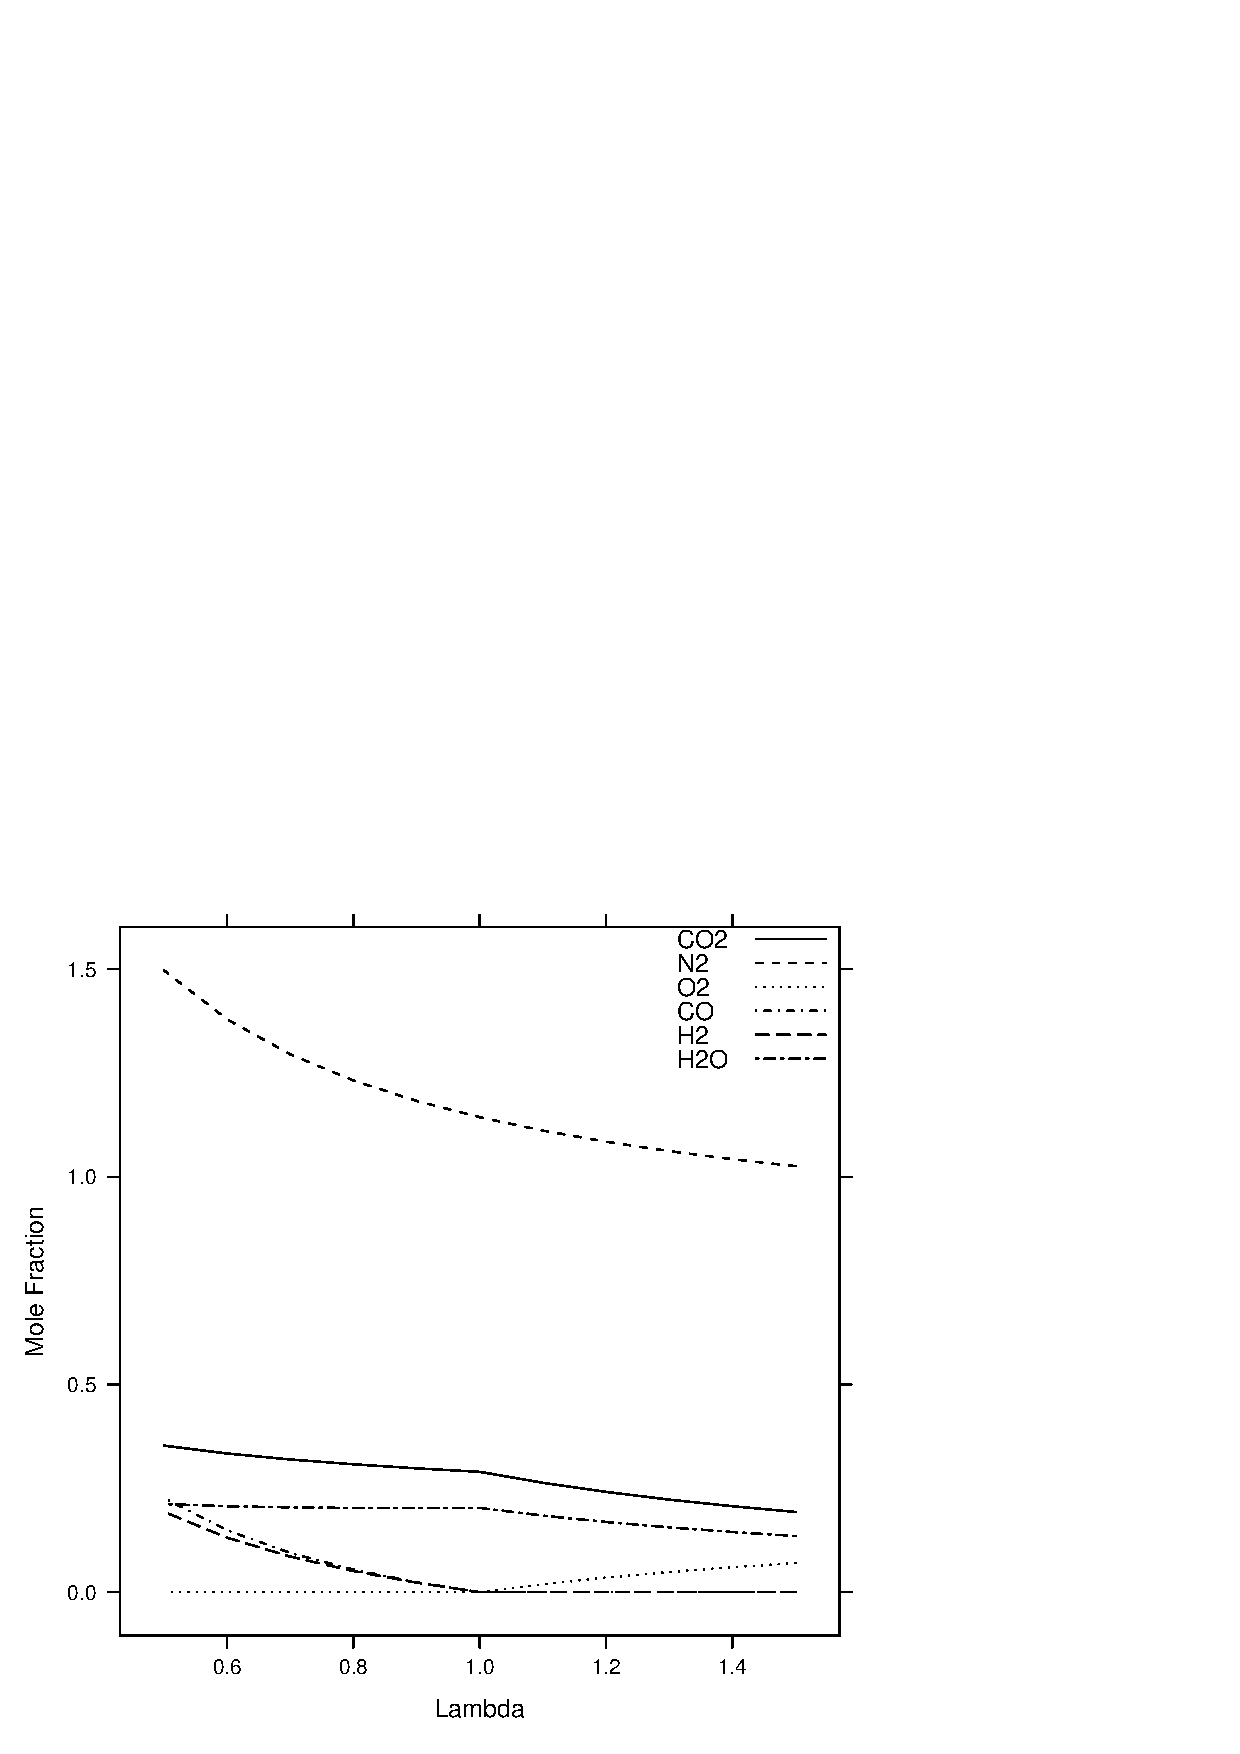
\includegraphics{images/img-007}
\\

\end{document}
